
\newsavebox{\boxA}
\savebox{\boxA} {

}

\begin{table*}[t]
\caption{Classification Characteristics}
\label{tab:ExampleClassification}
\begin{center}
    \begin{tabular}{|c|c|c|c|c|c||c|c|}
    \hline
     Name & Activities & Events & Gateways & Flows & Actors & CWP States & CWP Edges \\
     \hline
     \hline
     \facetoface & 8 & 3 & 5 & 20 & 1 & 5 & 5 \\
     \hline
     \buynsell & 9 & 13 & 8 & 28 & 4 & 5 & 5 \\
     \hline
     \phware & 10 & 13 & 8 & 38 & 3 & 6 & 6 \\
     \hline
     Sequential Scaling & 86 & 2 & 85 & 257 & 1 & 2 & 1 \\
     \hline
     Parallel Scaling & 12 & 12 & 6 & 30 & 6 & 2 & 1 \\
     \hline
    \end{tabular}
\end{center}
\end{table*}

\begin{table*}[t]
\caption{Verification Results}
\label{tab:VerificationResults}
\begin{center}
    \begin{tabular}{|c|c|c|c|c|c||c|}
    \hline
     Example Name & Most Difficult Property & States & Memory & Transitions & Time (S) & Total Time (M:S)\\
     \hline
     \hline
     \facetoface & NegotiationsEdges & 131 & 12KB & 284 & 2.29 & 0:26 \\
     \hline
     \buynsell & Purchase\textunderscore AgreedEdges & 712 & 79KB & 1984 & 2.95 & 0:33 \\
     \hline
     \phware & ptExpiredStateEdges & 90580 & 10MB & 792027 & 3.88 & 0:50 \\
     \hline
     Parallel Scaling & Init\textunderscore StateEdges & 7199431 & 824MB & 57522243 & 32.22 & 1:40 \\
     \hline
     Sequential Scaling & Init\textunderscore StateEdges & 1033 & 19KB & 2061 & 257.85 & 29:49 \\
     \hline
     
    \end{tabular}
\end{center}
\end{table*}

This tool has been used to verify five BPMN-CWP pairs. The effectiveness of this tool will be primarily measured by the verification time. Generally, verification time of a model increases with the presence of parallel actors, branching decision trees, and looping structures. The five examples are intended to show how effective the tool is at keeping verification time as low as possible given some or all of these conditions.
 
Although we consider readability to be a goal of this project, measuring it requires a usability study. A usability study is out of scope for this research and is left for future work. This section will focus on the primary metric - verification time.

The examples can be categorized into two groups. The first group is three case studies. These are \facetoface, which was explained in \secref{sec:simpleExample}. The next one is called \buynsell, which models a system for an online exchange of goods. The final one is \phware, which models a remote care procedure for patients with COVID-19.

The second group consists of two examples driven by scalability measures. The first is a sequential scaling example, which has a single actor performing many binary decisions in a row. Sequential decision making is a staple in workflows, and this example helps us understand the limits of sequential decisions using this automated verification tool. The second example is a parallel scaling example, which has many actors sharing a piece of shared memory. This introduces a large amount of interleaving, drastically increasing the required state space. It is common to have multiple actors in a workflow, and it can introduce much more complexity than expected. This example helps us understand the upper limit on the number of actors that can be verified using this tool.

Classification characteristics for the BPMN workflows and CWPs used in these five examples are found in \tabref{tab:ExampleClassification}. The values for parallel and sequential scaling are in reference to the largest examples verified. Additional details about each example, including workflow and CWP graphics, can be found in \appendixref{sec:evaluationExamples}.
\begin{comment}
\begin{figure*}[t]
  \begin{center}
    \begin{tabular}{c}
        \includesvg[inkscapeformat=png, width=\textwidth]{../figs/BPMN/face2face_May_5_2023_workflow.svg}
    \end{tabular}
  \end{center}
\caption{BPMN workflow for a face-to-face purchase with negotiations}
\label{fig:face2face_bpmn}
\end{figure*}

\begin{figure*}[t]
  \begin{center}
    \begin{tabular}{c}
        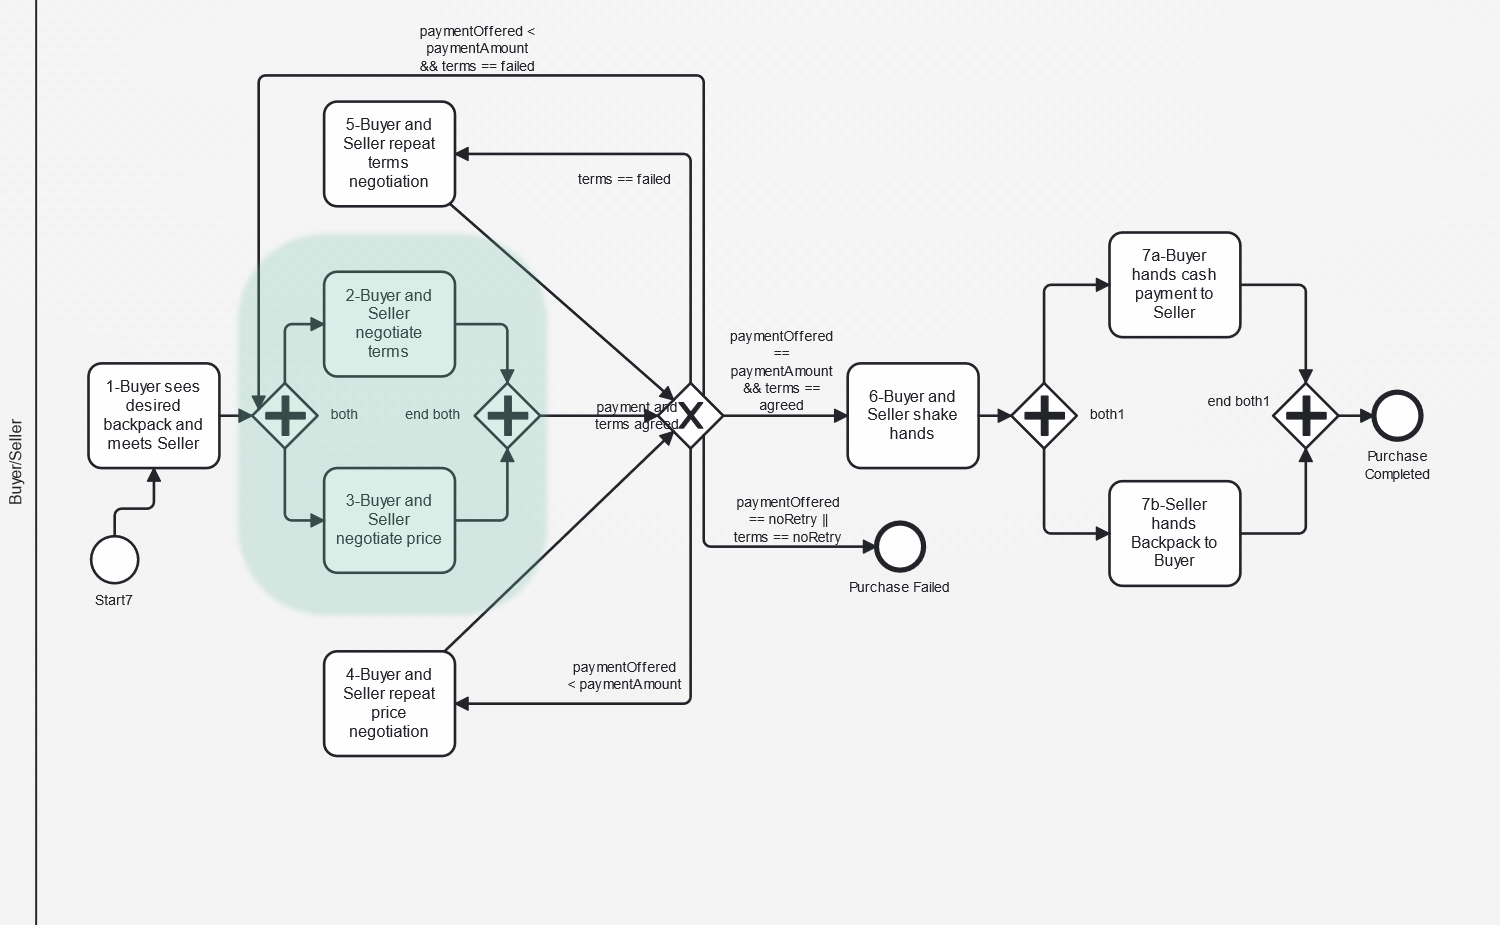
\includegraphics[width=\textwidth]{paper/figs/BPMN/face2face_May_5_2023_workflow_fixed.png}
    \end{tabular}
  \end{center}
\caption{Fixed BPMN workflow for a face-to-face purchase with negotiations. Fixed section highlighted in green.}
\label{fig:face2face_bpmn_fixed}
\end{figure*}
\end{comment}

\begin{comment}
\figref{fig:face2face_bpmn} shows the BPMN of the first example, a face-to-face purchase. The Buyer and seller are condensed into a single actor for simplicity in this model. The purchase process involves negotiation periods for both the price and the terms. Once the price and terms are agreed upon, the model can proceed to the exchange and then exit. \figref{fig:purchase_cwp} shows the CWP for this purchase. The CWP has 5 states, of which 2 are goal states. It is the workflow's responsibility to either send the state of the CWP to "Purchase Failed" or to "Ownerships Switched". Note that even though "Purchase Failed" might not sound like a goal state, it is for purposes of verifying eventual termination.
\end{comment}



Results of verification are found in \tabref{tab:VerificationResults}. The first column gives the example name. Columns two through six provide detailed results for the most time-consuming property to verify. These details include total states searched, memory used up by state storage, total transitions taken during verification, and time spent verifying that property. The final column gives total time to verify the entire example.

A few interesting points here. First is that of the case study examples, \phware~had the most explored states, memory used, transitions, and took the longest to verify. We believe this is because of the looping structure of the \phware~BPMN. The possibility of looping through the same activities multiple times increases complexity.

Next, looking at the scaling examples, we can see that although parallel scaling searched more states and required more memory than sequential scaling, it took significantly less time. Sequential scaling took almost 30 minutes complete with 85 decisions. The most difficult property took 257 seconds.  What's interesting is that it used up significantly less memory and searched fewer states than did parallel scaling. We believe this to be the result of a large upfront cost for generating the automata necessary for verification. This cost is particularly large for sequential scaling because of the number of elements in the BPMN. As seen in \tabref{tab:ExampleClassification}, sequential scaling has almost ten times the number of elements as other examples.

Two major actors in the BPM workspace, Camunda \cite{Camunda} and Bizagi\cite{Bizagi}, both encourage BPMN modelers to keep diagrams as compact and simple as possible. Also, a survey of over 800 business process models from three companies revealed that the average number of activities in a model was under ten \cite{BPMSizes}. A primary goal of BPMN as a standard is to provide easily readable and understandable visual models at a glance. If a model gets too large, it becomes difficult to read and understand. In those situations, it is best to identify parts of the model that can be separated into separate processes. Because of these recommendations, we believe that the results of our testing indicate that this model checking method scales sufficiently.

The left half of \figref{fig:ScalingVerificationTimes} shows the increase in verification time as the number of linear decisions increases in the sequential scaling BPMN example. The time requirement increases quadratically as the number of decisions increases. The largest example we tested had eighty-five (85) sequential steps and took about thirty minutes to complete verification.

\begin{figure*}[t]
  \begin{center}
    \begin{tabular}{cc}
        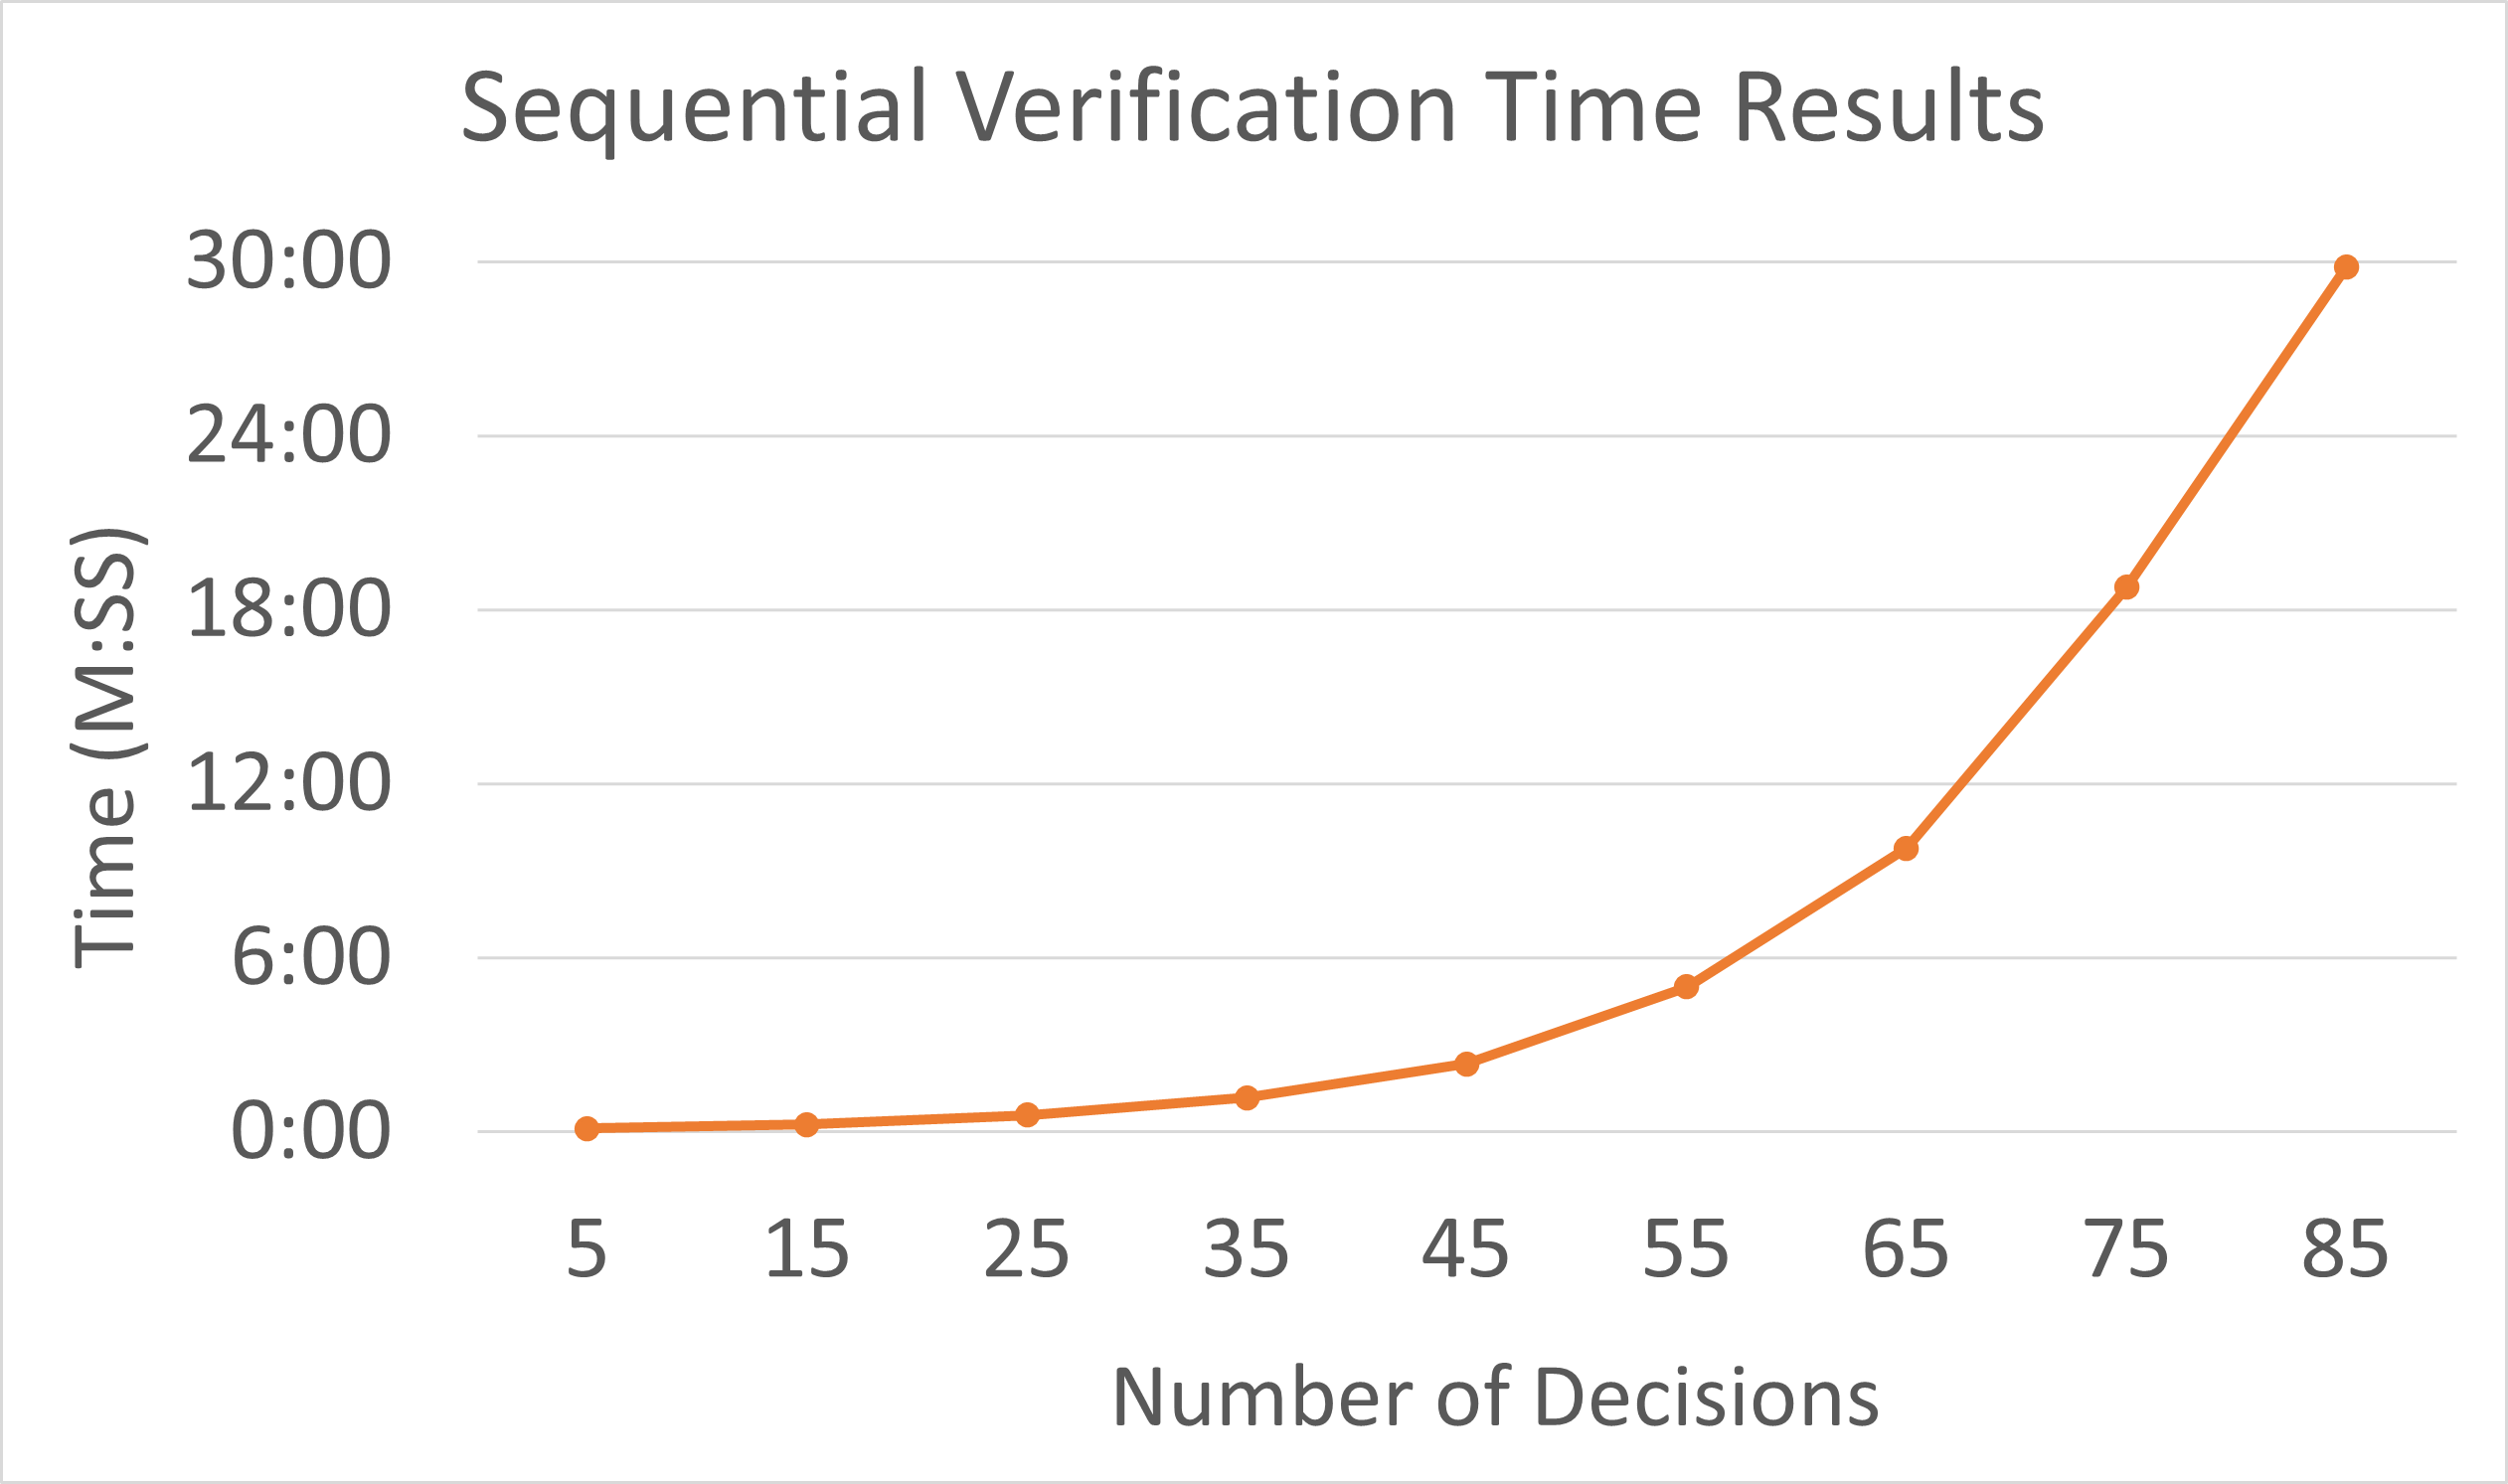
\includegraphics[width=.5\textwidth]{../figs/Data/Sequential_scaling_verification_times.png} &
        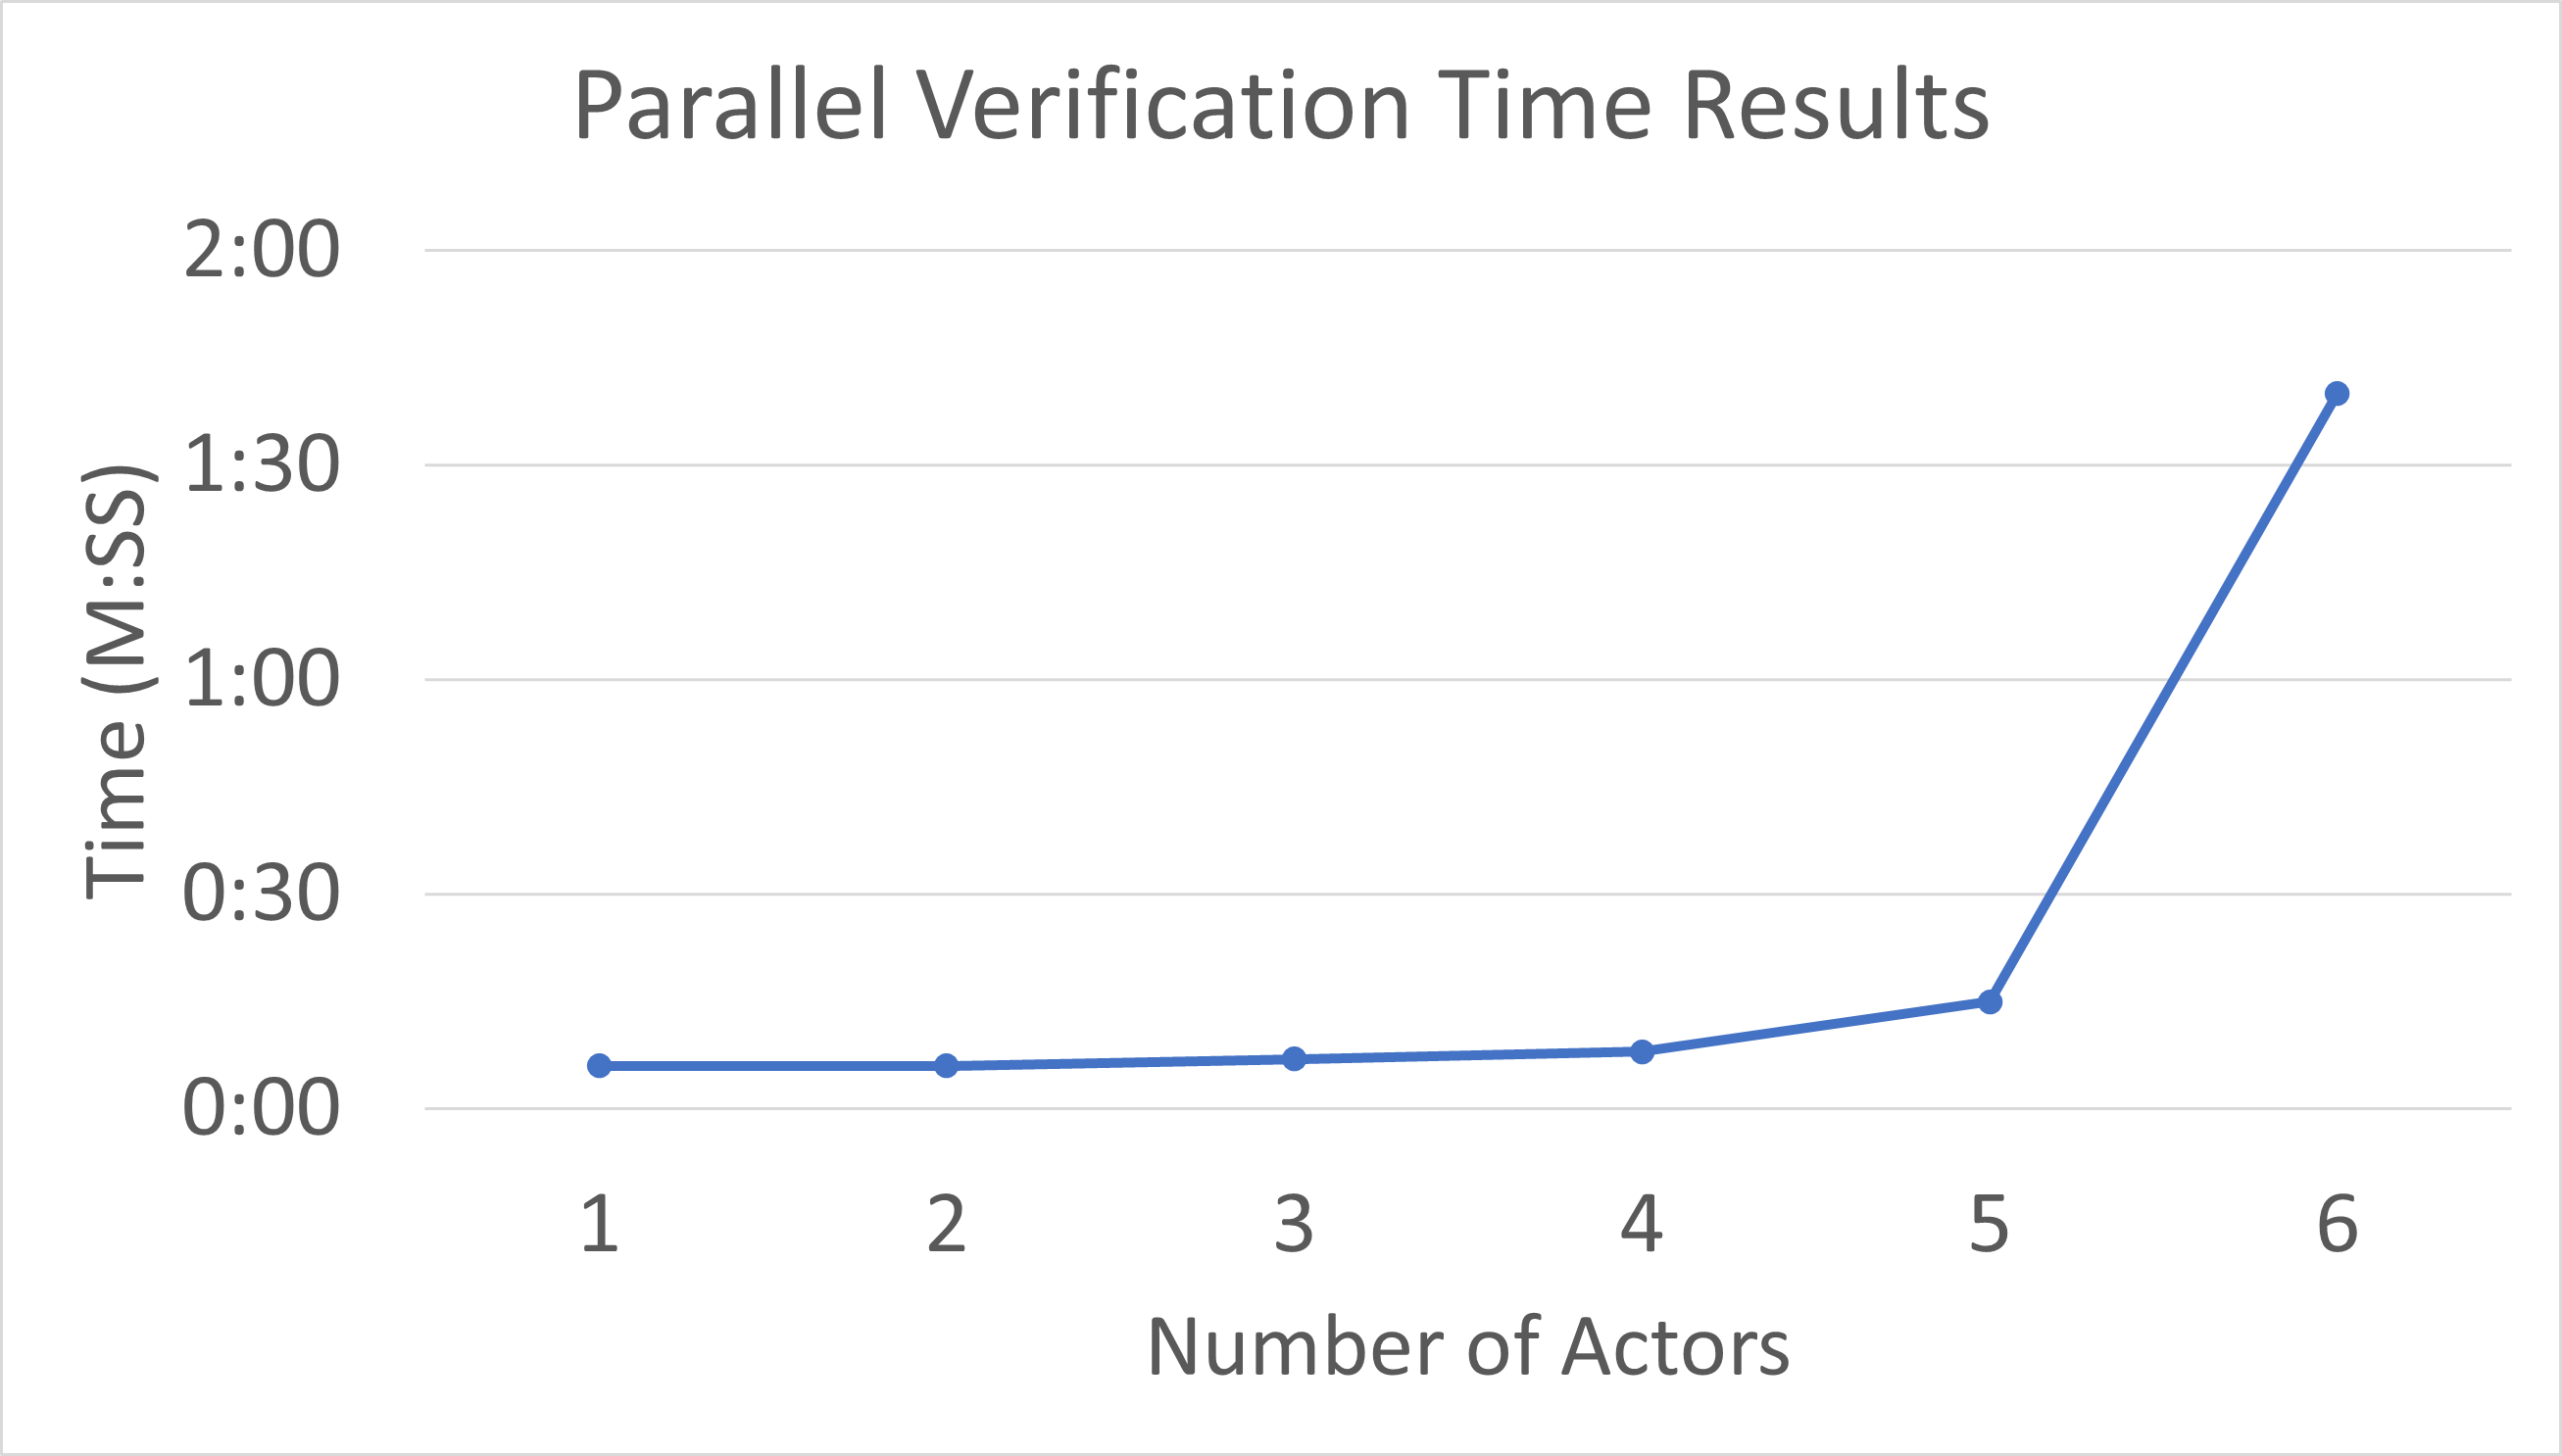
\includegraphics[width=.5\textwidth]{../figs/Data/Parallel_scaling_verification_times.png}
    \end{tabular}
  \end{center}
\caption{Verification times for the sequential and parallel scaling examples}
\label{fig:ScalingVerificationTimes}
\end{figure*}

The right half of \figref{fig:ScalingVerificationTimes} shows the increase in verification time as the number of asynchronous actors increases in the parallel scaling BPMN example. Although the increase in verification time increases exponentially with the number of actors, it is important to note that this parallel example is the absolute worst case scenario in terms of parallelization. The structure of the parallel scaling example was created to introduce the maximum possible number of race conditions. This results in an incredibly fast increase in the number of states the model checker must search through.
